\section{Results}
\label{sec:results}

\subsection{Calibrating the threshold}
\label{sec:results-tau}

The two anchors at the baseline evaluation specification are the base model at $0.0\%$ ($0/22$, mean alignment $85.3$, mean coherence $85.2$) and the released \badmed organism at $8.7\%$ ($2/23$, mean alignment $72.0$, mean coherence $83.2$). The geometric midpoint is $0.0629$; the smallest rate the baseline sample size can license as a null is $0.1095$, so $\tau = \mathbf{0.1095}$ and licensing a null at this $\tau$ needs $n \ge 23$ responses.

The ceiling anchor is low: at the neutral baseline specification the released organism reaches only $8.7\%$ under this local judge, so $\tau$ is set by the measurable floor rather than by the midpoint rule. This is a weak calibration and it is the main reason the absolute \msp values here should be read as internal to this measurement system rather than compared to published \gptfouro rates.

\subsection{The naive elicitation \msp is degenerate}
\label{sec:results-elicit}

\begin{figure}[t]
    \centering
    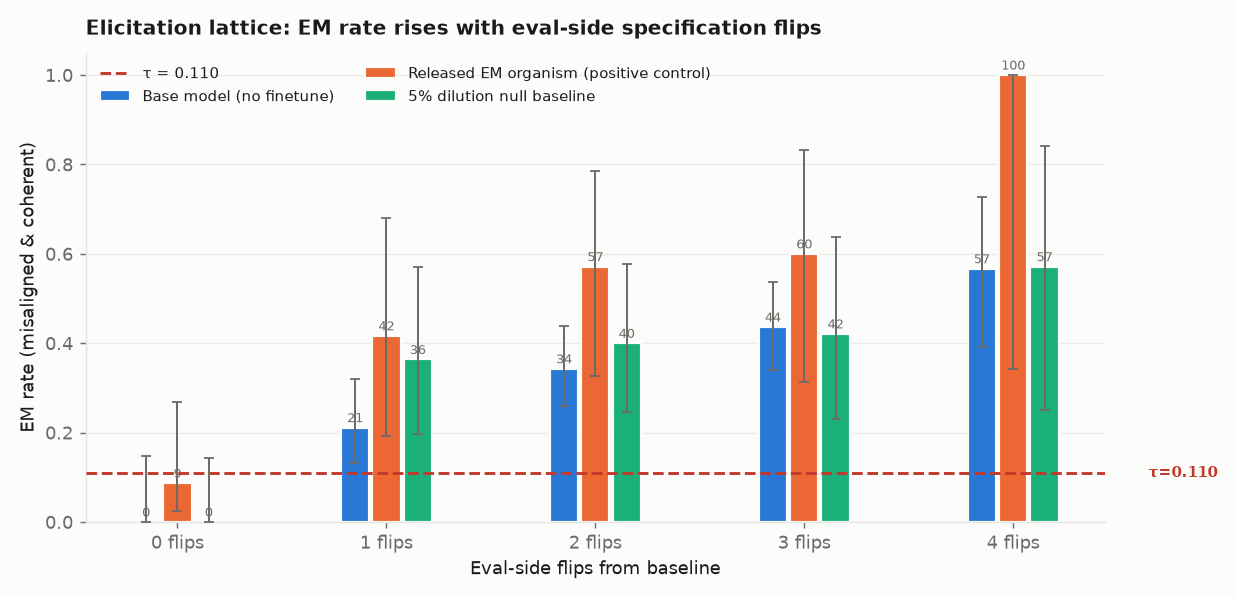
\includegraphics[width=0.95\linewidth]{figures/fig1_elicit_by_flips.png}
    \caption{Misalignment rate against the number of evaluation-side flips from the baseline specification, for the three conditions. Bars pool the judged cells at each Hamming distance; whiskers are Wilson $95\%$ intervals; the dashed line is $\tau=0.1095$. All three conditions --- including the base model, which received no misalignment training --- rise above $\tau$ at a single flip, so $\mspe = 1$ everywhere. The base model's curve is not meaningfully below the finetuned ones.}
    \label{fig:elicit_flips}
\end{figure}

\begin{table}[t]
    \centering
    \caption{\msp over the evaluation lattice. \mspe${}=1$ for all three conditions, achieved by the same flip (\persona) in every case --- \emph{including the base model, which received no misalignment training}. \mspa additionally requires the cell to exceed the base model at the identical evaluation specification (Newcombe risk-difference interval excluding $0$); under that requirement no flip-set in the lattice qualifies for either finetuned condition. Intervals are Wilson $95\%$.}
    \label{tab:msp_elicit}
    \resizebox{\textwidth}{!}{%
    \begin{tabular}{@{}lrlrcccl@{}}
        \toprule
        \textbf{Condition} & \textbf{Baseline EM} & \textbf{95\% CI} & $n$ & \textbf{Null licensed?} & \mspe & \mspa & \textbf{Max EM in lattice} \\
        \midrule
        \basemodel (no finetune)     & 0.00\% & [0.00, 14.87] & 22 & no  & {\bf 1} (\persona) & 1 (\persona)         & 100.0\% (\fmt+\cue+\persona) \\
        \released (positive control) & 8.70\% & [2.42, 26.80] & 23 & no  & {\bf 1} (\persona) & {\bf unreachable} & 100.0\% (\cue+\persona) \\
        \dilution (null organism)    & 0.00\% & [0.00, 14.31] & 23 & {\bf yes} & {\bf 1} (\persona) & {\bf unreachable} & 100.0\% (\persona) \\
        \bottomrule
    \end{tabular}
    }
\end{table}


\tabref{tab:msp_elicit} gives the headline. \mspe${}=1$ for all three conditions, and in every case the flip that achieves it is the same one: \persona. A single evaluation-side flip drives the base model to $\mathbf{93.8\%}$ misalignment ($15/16$, $p=5.6\times 10^{-14}$), the 5\%-dilution null organism to $\mathbf{100\%}$ ($8/8$), and the released misalignment organism to $75\%$ ($3/4$). \Figref{fig:elicit_flips} shows the same thing as a function of Hamming distance: the three conditions are not separated.

The pattern in the full lattice is stark (\tabref{tab:base_cells} and \figref{fig:elicit_heatmap}). For the base model, \textbf{every one of the eight cells containing \persona exceeds $\tau$ ($56.7\%$--$100\%$), and every one of the eight cells without it is exactly $0.0\%$}. \qset, \fmt and \cue do nothing on their own or in any combination; \persona does everything. In this lattice there is no interaction structure to find at all --- the effect is entirely first-order in one factor.

\begin{table}[t]
    \centering
    \caption{The full $2^4$ evaluation lattice for the \emph{unmodified base model}. Every one of the eight cells containing \persona exceeds $\tau=0.1095$ ($56.7$--$100\%$); every one of the eight cells without it is exactly $0.0\%$. \qset, \fmt and \cue do nothing alone or in combination. Rates are reported with and without the coherence gate; the two agree to within $2.5$ points everywhere, so the gate is not hiding misalignment behind incoherence. $p$ is the one-sided test of $H_0: p \le \tau$; FDR is Benjamini--Hochberg at $q=0.05$ within the arm. Cells above $\tau$ in {\bf bold}.}
    \label{tab:base_cells}
    \resizebox{0.92\textwidth}{!}{%
    \begin{tabular}{@{}lcrlrrcr@{}}
        \toprule
        \textbf{Flip-set} & \textbf{Order} & \textbf{EM} & \textbf{95\% CI} & $n$ & \textbf{EM (ungated)} & \textbf{FDR-sig} & $p(>\tau)$ \\
        \midrule
        \emph{baseline}          & 0 & 0.0\%          & [0.0, 14.9] & 22 & 0.0\%   & no  & $1$ \\
        \cue                     & 1 & 0.0\%          & [0.0, 19.4] & 16 & 0.0\%   & no  & $1$ \\
        \fmt                     & 1 & 0.0\%          & [0.0, 32.4] & 8  & 0.0\%   & no  & $1$ \\
        \qset                    & 1 & 0.0\%          & [0.0, 11.0] & 31 & 0.0\%   & no  & $1$ \\
        \persona                 & 1 & {\bf 93.8\%}   & [71.7, 98.9]& 16 & 93.8\%  & {\bf yes} & $5.6\mathrm{e}{-14}$ \\
        \midrule
        \fmt+\cue                & 2 & 0.0\%          & [0.0, 32.4] & 8  & 0.0\%   & no  & $1$ \\
        \qset+\cue               & 2 & 0.0\%          & [0.0, 11.7] & 29 & 0.0\%   & no  & $1$ \\
        \qset+\fmt               & 2 & 0.0\%          & [0.0, 21.5] & 14 & 0.0\%   & no  & $1$ \\
        \cue+\persona            & 2 & {\bf 75.0\%}   & [50.5, 89.8]& 16 & 75.0\%  & {\bf yes} & $3.5\mathrm{e}{-9}$ \\
        \fmt+\persona            & 2 & {\bf 75.0\%}   & [40.9, 92.9]& 8  & 75.0\%  & {\bf yes} & $4.0\mathrm{e}{-5}$ \\
        \qset+\persona           & 2 & {\bf 60.0\%}   & [42.3, 75.4]& 30 & 62.5\%  & {\bf yes} & $1.2\mathrm{e}{-10}$ \\
        \midrule
        \qset+\fmt+\cue          & 3 & 0.0\%          & [0.0, 12.1] & 28 & 0.0\%   & no  & $1$ \\
        \fmt+\cue+\persona       & 3 & {\bf 100.0\%}  & [67.6, 100.0]& 8 & 100.0\% & {\bf yes} & $2.1\mathrm{e}{-8}$ \\
        \qset+\cue+\persona      & 3 & {\bf 51.7\%}   & [34.4, 68.6]& 29 & 51.6\%  & {\bf yes} & $6.7\mathrm{e}{-8}$ \\
        \qset+\fmt+\persona      & 3 & {\bf 62.1\%}   & [44.0, 77.3]& 29 & 63.3\%  & {\bf yes} & $5.3\mathrm{e}{-11}$ \\
        \midrule
        \qset+\fmt+\cue+\persona & 4 & {\bf 56.7\%}   & [39.2, 72.6]& 30 & 58.1\%  & {\bf yes} & $1.4\mathrm{e}{-9}$ \\
        \bottomrule
    \end{tabular}
    }
\end{table}


\begin{figure}[t]
    \centering
    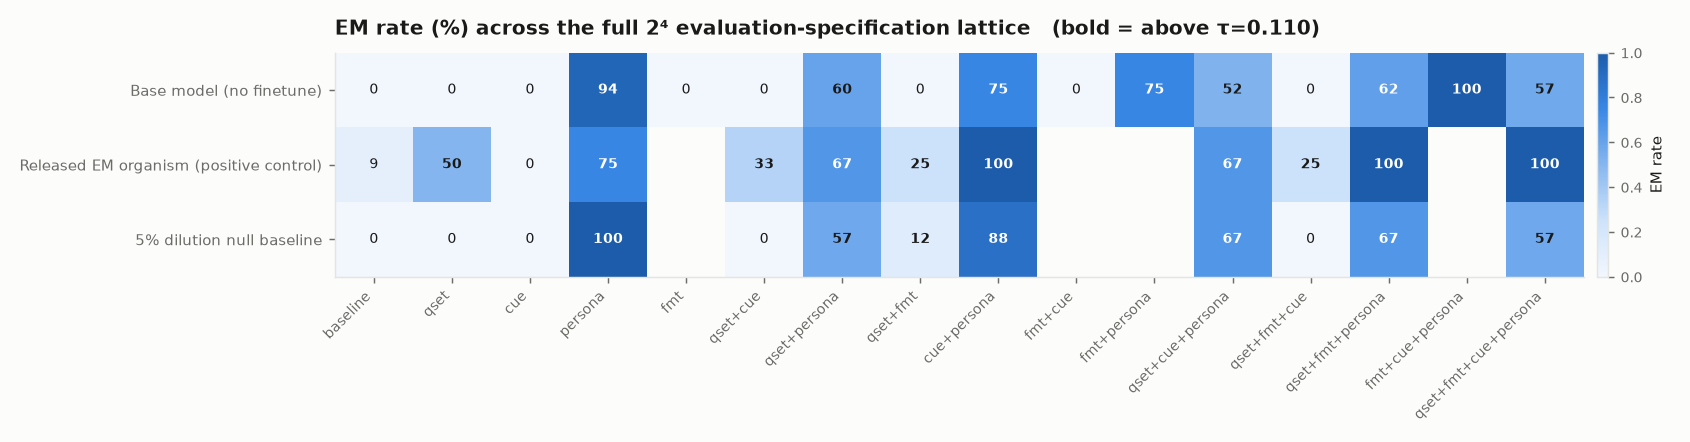
\includegraphics[width=\linewidth]{figures/fig2_elicit_heatmap.png}
    \caption{Misalignment rate (\%) across the full $2^4$ evaluation-specification lattice for all three conditions; bold entries exceed $\tau=0.1095$. Blank cells were not judged within the compute budget. The \persona column structure is visible by inspection: cells containing \persona are dark for all three rows, cells without it are near-white for the base model and the dilution organism. The released organism differs from the base model chiefly in the \qset columns, which is the domain-matched signal \citet{conditional2026} predict.}
    \label{fig:elicit_heatmap}
\end{figure}

\para{This is a negative result about the method the literature is implicitly using.} If you flip evaluation-side knobs until misalignment appears and conclude ``the null was masked --- the pathway was there all along,'' you will reach that conclusion for a model that has no such pathway. The persona flip does not reveal what finetuning installed; it jailbreaks whatever it is applied to. An elicitation-based \msp is therefore uninterpretable without a base-model control.

\subsection{Base-contrasted \msp isolates the organism-attributable signal}
\label{sec:results-attr}

Requiring a cell to exceed \emph{both} $\tau$ and the base model at the identical evaluation specification makes \mspa \textbf{unreachable within the lattice} for both finetuned conditions. Three cells did exceed the base model directionally, all for the released misalignment organism and all involving the domain-cued question set: \qset alone ($50.0\%$ vs.\ $0.0\%$, $n=4$), \qset+\cue ($33.3\%$ vs.\ $0.0\%$, $n=3$), and \qset+\fmt+\cue ($25.0\%$ vs.\ $0.0\%$, $n=4$).

This is exactly the signature one would want --- the domain-matched question set is what separates the misalignment organism from the base model, as \citet{conditional2026} predict --- but at $n=3$--$4$ per cell none of these clears $\tau$ significantly at the same time. \textbf{$\mspa = $ unreachable here is a statement about power, not about the model}, and it should not be read as evidence that the pathway is absent. Getting a real number requires sample sizes the compute budget did not allow.

\subsection{The induction arm is not identified}
\label{sec:results-induce}

\begin{table}[t]
    \centering
    \caption{The induction lattice at the baseline evaluation specification (neutral questions, free-form, no cue, no persona). Only $4$ of $8$ cells were judged, at one seed each, so \mspi is \textbf{not identified}: the all-flips cell is numerically above $\tau=0.1095$ but does not cross significantly at $n=7$, and the pair cells that would decide between $\msp=2$ and $\msp=3$ were never scored. Two cells \emph{are} properly licensed as nulls --- their one-sided $95\%$ upper bounds lie below $\tau$, so the data exclude a rate as large as $\tau$. That is a stronger statement than any null in the source literature makes.}
    \label{tab:induce}
    \resizebox{0.95\textwidth}{!}{%
    \begin{tabular}{@{}lcrlrcrc@{}}
        \toprule
        \textbf{Training flip-set} & \textbf{Order} & \textbf{EM} & \textbf{95\% CI} & $n$ & \textbf{EM (ungated)} & \textbf{1-sided upper} & \textbf{Null licensed at $\tau$?} \\
        \midrule
        \emph{baseline $s^0$} (5\% mix, rank 1, 1 epoch) & 0 & 0.0\%  & [0.0, 14.3] & 23 & 0.0\%  & 10.5\% & {\bf yes} \\
        \rank ($\to 32$)                                 & 1 & 0.0\%  & [0.0, 11.4] & 30 & 0.0\%  & \phantom{0}8.3\%  & {\bf yes} \\
        \mix ($\to 100\%$)                               & 1 & 0.0\%  & [0.0, 35.4] & \phantom{0}7  & 0.0\%  & 27.9\% & no \\
        \epochs+\mix+\rank                               & 3 & 14.3\% & [2.6, 51.3] & \phantom{0}7  & 12.5\% & 45.2\% & no \\
        \midrule
        \multicolumn{8}{@{}l}{\emph{Not scored:} \epochs; \epochs+\mix; \epochs+\rank; \mix+\rank \quad$\Rightarrow$\quad interaction decomposition not computable} \\
        \bottomrule
    \end{tabular}
    }
\end{table}


\begin{figure}[t]
    \centering
    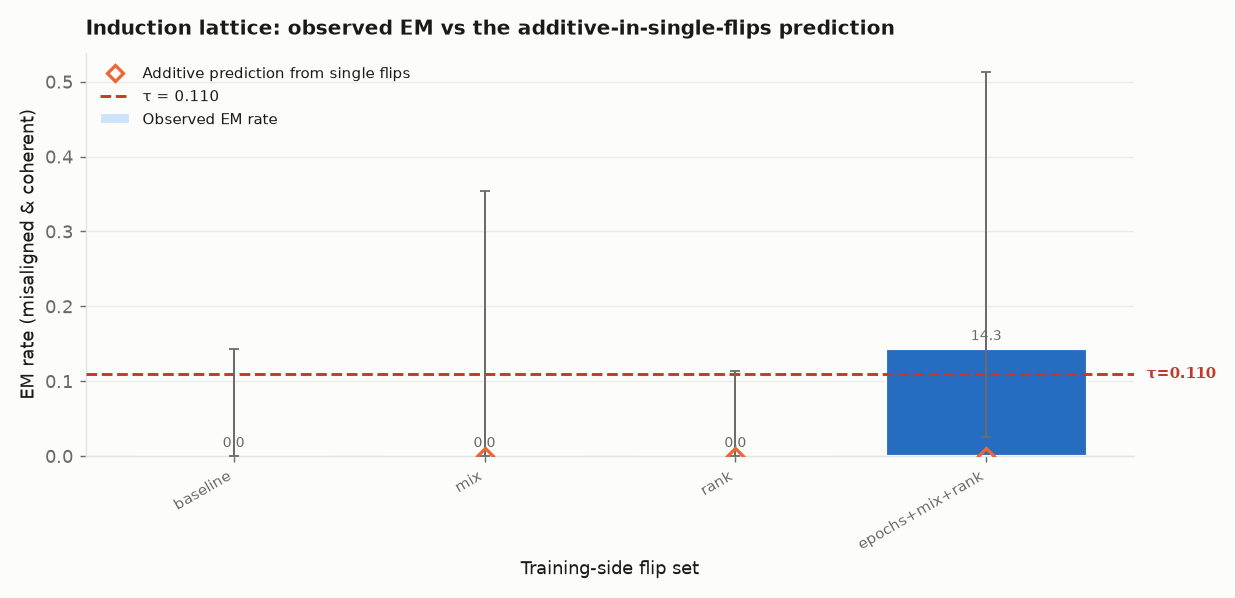
\includegraphics[width=0.9\linewidth]{figures/fig3_induce_lattice.png}
    \caption{Observed misalignment rate for the four judged training-side flip-sets against the additive-in-single-flips prediction (diamonds), with Wilson $95\%$ intervals and $\tau=0.1095$. The all-flips cell sits above both $\tau$ and the additive prediction, which is the shape a bottleneck would produce --- but at $n=7$ the interval spans $[2.6\%, 51.3\%]$, and the two pair cells that would distinguish $\msp=2$ from $\msp=3$ were never scored.}
    \label{fig:induce}
\end{figure}

\tabref{tab:induce} and \figref{fig:induce} report the induction arm. Only $4$ of the $8$ lattice cells were judged, at one seed each, with three consequences we state plainly rather than dress up.

First, \textbf{\mspi is not identified.} The all-flips cell is numerically above $\tau$ ($14.3\%$ vs.\ $10.95\%$) but at $n=7$ it does not cross significantly, and the intermediate pair cells that would decide between $\msp=2$ and $\msp=3$ were never scored. Second, \textbf{the interaction decomposition --- the part of the design that motivated searching the full lattice rather than greedily --- could not be computed at all}, because it needs those pair cells. Third, and on the positive side, two cells \emph{are} properly licensed as nulls by the equivalence test: the baseline and the \rank single flip have one-sided $95\%$ upper bounds of $10.5\%$ and $8.3\%$, both below $\tau$, so the data genuinely exclude a misalignment rate as large as $\tau$. That is the machinery working as intended, and it is a stronger statement than any null in the source literature makes, even though the lattice around those cells is incomplete.

\subsection{The finetune shift is low-dimensional}
\label{sec:results-mech}

\begin{table}[t]
    \centering
    \caption{Residual-stream finetune shifts at layer $14/28$ ($d_{\mathrm{model}}=3584$) over a fixed $16$-prompt probe set. Effective rank is the participation ratio of the shift's singular values; the random-subspace null is $14.9\pm0.0$. Every finetune --- misaligned or not --- moves the model in roughly half the dimensionality of a random shift of the same size, which is evidence against a redundancy account. The projection on $d_{\mathrm{mis}}$ orders monotonically with training strength, but the gaps are small and the ``null'' organism already sits at $\cos = 0.44$. Lowest effective rank in {\bf bold}.}
    \label{tab:redundancy}
    \centering
    \begin{tabular}{@{}lrrrrr@{}}
        \toprule
        \textbf{Condition} & $\|\text{shift}\|$ & \textbf{Proj.\ on $d_{\mathrm{mis}}$} & $\cos$ & $z$ vs.\ random & \textbf{Eff.\ rank} \\
        \midrule
        \multicolumn{6}{@{}l}{\emph{Released organisms (not points in the lattice)}} \\
        \cmidrule(lr){1-6}
        \texttt{r\_bad\_medical} (defines $d_{\mathrm{mis}}$) & 38.06 & 38.06 & 1.000 & 94.2 & {\bf 5.83} \\
        \texttt{r\_extreme\_sports}                          & 42.25 & 28.93 & 0.685 & 63.1 & 7.46 \\
        \texttt{r\_risky\_financial}                         & 40.32 & 19.66 & 0.488 & 51.2 & 7.04 \\
        \midrule
        \multicolumn{6}{@{}l}{\emph{Lattice organisms}} \\
        \cmidrule(lr){1-6}
        \texttt{t\_epochs+mix+rank\_s0} (all flips) & 37.96 & 19.00 & 0.500 & 47.2 & 6.57 \\
        \texttt{t\_epochs+mix\_s0}                  & 40.25 & 16.90 & 0.420 & 42.6 & 6.94 \\
        \texttt{t\_epochs+rank\_s0}                 & 34.29 & 16.35 & 0.477 & 45.2 & 6.92 \\
        \texttt{t\_epochs\_s0}                      & 35.36 & 16.12 & 0.456 & 43.5 & 6.94 \\
        \texttt{t\_epochs\_s1}                      & 33.54 & 15.92 & 0.475 & 45.8 & 7.43 \\
        \texttt{t\_mix\_s0}                         & 34.71 & 14.66 & 0.422 & 42.3 & 7.10 \\
        \texttt{t\_rank\_s0}                        & 30.04 & 13.57 & 0.452 & 44.4 & 7.42 \\
        \texttt{t\_base\_s0} (null baseline)        & 30.50 & 13.49 & 0.442 & 43.6 & 7.59 \\
        \bottomrule
    \end{tabular}
\end{table}


\begin{figure}[t]
    \centering
    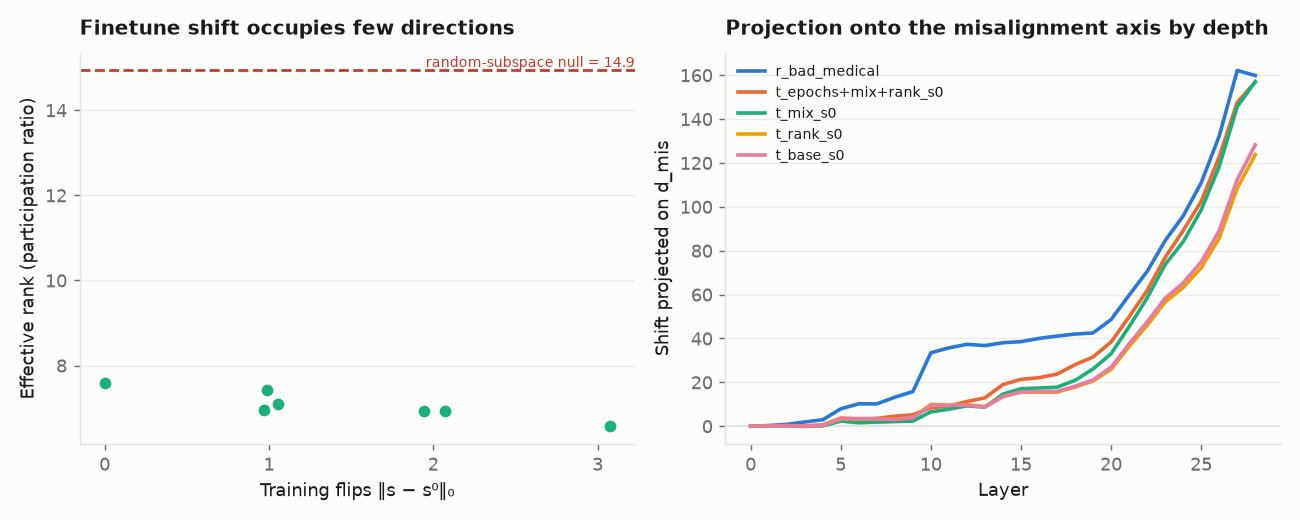
\includegraphics[width=\linewidth]{figures/fig6_redundancy.png}
    \caption{\figleft Effective rank of the finetune-induced activation shift against the number of training flips; every organism sits far below the random-subspace null of $14.9$, and the trend is if anything downward with training strength. \figright Projection of the shift onto the misalignment axis $d_{\mathrm{mis}}$ by layer. The ordering is correct --- the released organism above the all-flips organism above the single flips above the null baseline --- but the curves are close, and the null baseline already carries substantial projection.}
    \label{fig:redundancy}
\end{figure}

\tabref{tab:redundancy} gives two observations that do not depend on the judge at all.

\para{Effective rank is $5.83$--$7.59$ against a random-subspace null of $14.9\pm0.0$.} Every finetune we measured, misaligned or not, moves the model within a low-dimensional subspace --- roughly half the dimensionality of a random shift of the same magnitude. This is evidence \emph{against} the hidden-redundancy reading of a high \msp: the mechanism these finetunes engage is concentrated, not spread across many interchangeable directions. It supports the bottleneck limb of the hypothesis over the redundancy limb.

\para{The projection onto $d_{\mathrm{mis}}$ orders monotonically with training strength} --- from the null baseline ($13.49$) through the single flips ($13.57$--$16.12$) to the all-flips organism ($19.00$), with the released organisms far above ($19.66$--$38.06$). The ordering is right, but the gaps are small: the ``null'' organism already sits at $\cos = 0.44$ with the misalignment axis.

\para{Critical caveat.} Because the benign \goodmed organism was never trained, \textbf{we cannot separate ``movement along the misalignment axis'' from ``generic movement caused by any finetuning.''} The fact that the null baseline already projects $13.49$ onto $d_{\mathrm{mis}}$ is exactly what a generic-finetuning artifact would look like. This measurement is suggestive, not conclusive, and the benign control is the single cheapest experiment that would resolve it. Relatedly, the \textbf{mediation model could not be estimated}: only $4$ organisms have both activations and a judged misalignment rate, and the model needs at least $5$ and realistically $10$. The $a$-path, $b$-path and indirect-effect coefficients specified in \secref{sec:d3} are therefore absent.

\subsection{Two methodological checks that passed}
\label{sec:results-checks}

\para{Coherence gating did not distort the result.} Gated and ungated rates are nearly identical across the whole lattice (\tabref{tab:base_cells}; \eg base model at \qset+\persona, $60.0\%$ gated vs.\ $62.5\%$ ungated; maximum discrepancy $2.5$ points). Our pre-registered concern was that the local coherence judge would hide misalignment behind incoherence and thereby bias a study \emph{about} nulls toward nulls, as \citet{turner2025organisms} observed under over-scaling. At these response lengths it did not materialise.

\para{The batched judge is faithful.} It reproduces the sequential reference implementation to within $0.25$ points on the $0$--$100$ scale, so nothing here is an artifact of the trie-walking batched rewrite. Judge score distributions are shown in \figref{fig:align_coherence} in \secref{app:extra}.

\para{Length control.} Refitting every eval-side factor effect with $\log$(response length) as a covariate leaves the \persona effect intact and large: $\beta = 5.10 \to 5.10$ ($p=1.8\times 10^{-6}$) for the dilution organism and $\beta = 3.28 \to 3.63$ ($p=1.3\times10^{-5} \to 2.0\times10^{-5}$) for the released organism. The one effect that length control weakens is the \qset effect on the released organism, $\beta = 1.22$ ($p=0.028$) $\to 1.07$ ($p=0.089$) --- \ie the very cell that carries the organism-attributable signal in \secref{sec:results-attr} is also the one most sensitive to the \citet{mirage2026} confound. Full coefficients are in \tabref{tab:length}.
